\documentclass[aspectratio=169]{beamer}

%%% Работа с русским языком
\usepackage{cmap}					% поиск в PDF
\usepackage{mathtext} 				% русские буквы в формулах
\usepackage[T2A]{fontenc}			% кодировка
\usepackage[utf8]{inputenc}			% кодировка исходного текста
\usepackage[english,russian]{babel}	% локализация и переносы
\usepackage{indentfirst}
\frenchspacing

%%% Дополнительная работа с математикой
\usepackage{amsmath,amsfonts,amssymb,amsthm,mathtools} % AMS
\usepackage{icomma}

%%% Текст в колонки
\usepackage{multicol}

%%% Системы уравнений
\usepackage{cases}

%%% Таблицы
\usepackage{array}
\usepackage{../slashbox}

%%% Картинки
\usepackage{graphicx}
\usepackage{float}

%%% Свои имена функций
\DeclareMathOperator{\Div}{div}
\DeclareMathOperator{\Const}{const}

%%% Список литературы
\usepackage[sorting=none]{biblatex}
\addbibresource{../references.bib}

%%% Гиперссылки
\usepackage{hyperref}

%%% Перенос знаков в формулах (по Львовскому)
\newcommand*{\hm}[1]{#1\nobreak\discretionary{}
{\hbox{$\mathsurround=0pt #1$}}{}}

%%% Цвета
\definecolor{red}{RGB}{200,0,0}


\usetheme{Madrid}
\title[Электрический пробой]{Исследование модели диффузной границы для развития канала
	электрического пробоя}
\author{
	\raggedright
	\hfill \break
	\hspace*{8cm}
	\textbf{Студент:} \linebreak
	\hspace*{8cm}
	\vspace{0.3cm}
	Пономарев Андрей Сергеевич \linebreak
	\hspace*{8cm}
	\textbf{Научный руководитель:} \linebreak
	\hspace*{8cm}
	\vspace{0.3cm}
	Савенков Евгений Борисович
	\hspace*{8cm}
	\textbf{Консультант:} \linebreak
	\hspace*{8cm}
	Зипунова Елизавета Вячеславовна
}
\date[]{20.06.2024}
\logo{
\includegraphics[height=0.8cm]{../figures/labels.jpg}}


\begin{document}

\AtBeginSection[]{
	\begin{frame}{Содержание}
	\Large
	\tableofcontents[currentsection]
	\end{frame}
}


\begin{frame}
\titlepage
\end{frame}


\begin{frame}{Содержание}
\Large
\tableofcontents
\end{frame}


\section{Введение}

\begin{frame}{Физическое явление}
\begin{block}{Электрический пробой}
	Явление резкого возрастания тока в диэлектрике при приложении электрического напряжения
	выше критического.
\end{block}
\begin{itemize}
	\item Рассматриваем твердый диэлектрик
	\item Деградация диэлектрических свойств материала
	\item Процесс развивается в ограниченной зоне -- канале пробоя
	\item Сложная физическая природа
\end{itemize}
\end{frame}


\begin{frame}{Математическая модель}
\begin{block}{Модель типа диффузной границы}
	Вещество находится в разных фазах. Состояние вещества описывается гладкой функцией
	$\phi(\textbf{x}, t)$ -- фазовым полем.
\end{block}
\begin{itemize}
	\item $\phi = 1$ -- неповрежденная среда
	\item $\phi = 0$ -- полностью разрушенная среда
	\item Зона $\phi \in (0, 1)$ -- диффузная граница
	\item На разрушение среды тратится энергия
\end{itemize}
\begin{figure}
	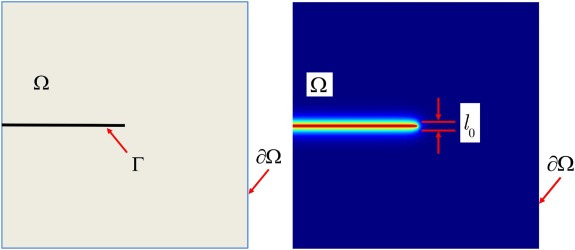
\includegraphics[width=0.5\textwidth]{../figures/diffuse_edge.jpg}
\end{figure}
\end{frame}


\begin{frame}{Математическая модель}
Модель, предложенная в работе \cite{pitike_dielectric_breakdown}:
\begin{itemize}
	\item $\pi = \textcolor{red}{-\cfrac{1}{2} \epsilon[\phi] (\nabla \Phi, \nabla \Phi)} +
	\Gamma \left( \cfrac{1 - f(\phi)}{l^2} + \cfrac{1}{4} (\nabla \phi, \nabla \phi) \right)$
	-- плотность свободной энергии
	\item $\Gamma$ -- энегрия роста пробоя на единицу длины
	\item $l$ -- величина <<размытия>> пробоя
	\item $\epsilon(\textbf{x}, t)$ -- диэлектрическая проницаемость среды
	\item $f(\phi)$ -- интерполирующая функция
\end{itemize}
\end{frame}


\begin{frame}{Математическая модель}
\vspace{-0.2cm}
\begin{itemize}
	\item $\epsilon(\textbf{x}, t) = \cfrac{\epsilon_0(\textbf{x})}{f(\phi(\textbf{x}, t)) +
	\delta}$ -- диэлектрическая проницаемость среды
	\item $f(\phi) = 4 \phi^3 - 3 \phi^4$ -- интерполирующая функция
\end{itemize}
\begin{columns}
\column{0.5\textwidth}
\begin{figure}
	\hspace*{1.4cm}
	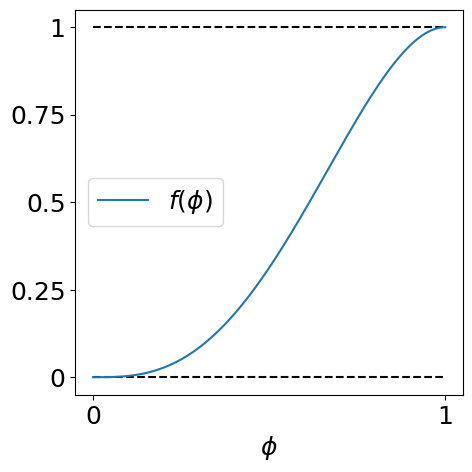
\includegraphics[width=0.65\textwidth]{../figures/f_form.png}
\end{figure}
\column{0.5\textwidth}
\begin{figure}
	\hspace*{-2cm}
	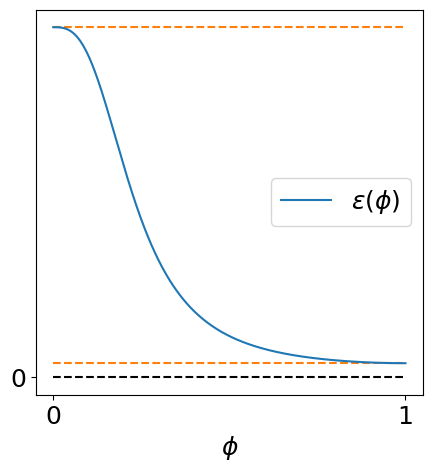
\includegraphics[width=0.60\textwidth]{../figures/eps_form.png}
\end{figure}
\end{columns}
\end{frame}


\begin{frame}{Математическая модель}
\vspace{-0.5cm}
\begin{block}{Уравнения модели}
\begin{itemize}
	\item Уравнение электрического потенциала $\Phi$:
	\begin{equation}
		\Div(\epsilon[\phi] \nabla \Phi) = 0
		\label{equation_potential}
	\end{equation}
	\item Уравнение фазового поля $\phi$:
	\begin{equation}
		\cfrac{1}{m} \cfrac{\partial \phi}{\partial t} = \cfrac{1}{2} \epsilon'(\phi)
		(\nabla \Phi, \nabla \Phi) + \cfrac{\Gamma}{l^2} f'(\phi) +
		\cfrac{1}{2} \Gamma \triangle \phi
		\label{equation_phase}
	\end{equation}
\end{itemize}
\end{block}
Свойства:
\begin{itemize}
	\item связанная система уравнений на $\phi$ и $\Phi$;
	\item уравнение для $\phi$ типа Аллена--Кана, нелинейное.
\end{itemize}
\end{frame}


\begin{frame}{Пример вычислительного эксперимента}
\begin{columns}
\column{0.32\textwidth}
\begin{figure}
	
\includegraphics[width=\textwidth]{../figures/model_example_1.png}
\end{figure}
\column{0.32\textwidth}
\begin{figure}
	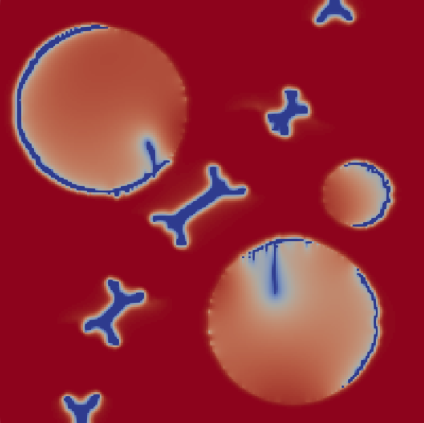
\includegraphics[width=\textwidth]{../figures/model_example_2.png}
\end{figure}
\column{0.32\textwidth}
\begin{figure}
	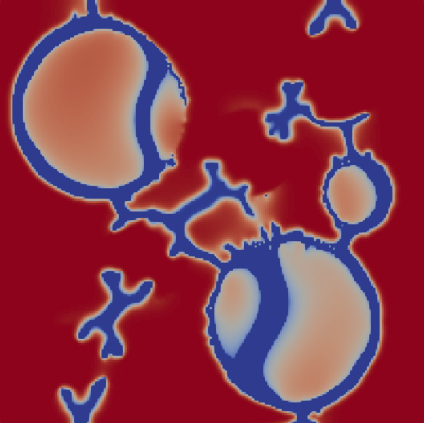
\includegraphics[width=\textwidth]{../figures/model_example_3.png}
\end{figure}
\end{columns}
\begin{center}
	Расчет из работы \cite{zipunova_experiment}
\end{center}
\end{frame}


\begin{frame}{Цель работы}
\begin{block}{Цель работы}
	Исследовать качественные характеристики системы уравнений \eqref{equation_potential},
	\eqref{equation_phase}: условия развития канала пробоя, границы применения разностной
	схемы.
\end{block}
Для этого будем рассматривать задачу в определенных краевых условиях, упрощающих ее, но
позволяющих установить интересующие нас свойства.
\end{frame}


\section{Постановка задачи}

\begin{frame}{Одномерная задача}
\vspace{-0.3cm}
\begin{itemize}
	\item Область $\Omega = [0, w]_x \times [0, h]_y \times I_z$ в форме параллелепипеда;
	\item $\phi(\textbf{x}, 0) = \phi_0(\textbf{x}) = \phi_0(x), \; \epsilon_0(\textbf{x}) =
	\epsilon_0(x)$ не зависят от $y$ и $z$;
	\item $\Phi|_{y = 0} = \Phi^- \in \mathbb{R}, \; \Phi|_{y = h} = \Phi^+ \in \mathbb{R}$.
\end{itemize}
\vspace{0.3cm}
Решением является функция электрического потенциала
\begin{columns}
\column{0.65\textwidth}
\vspace{-1cm}
$$\Phi(\textbf{x}, t) = \Phi^- \hm + \cfrac{y}{h}(\Phi^+ - \Phi^-)$$
\column{0.35\textwidth}
\begin{figure}
	\vspace*{-2cm}
	\hspace*{0.5cm}
	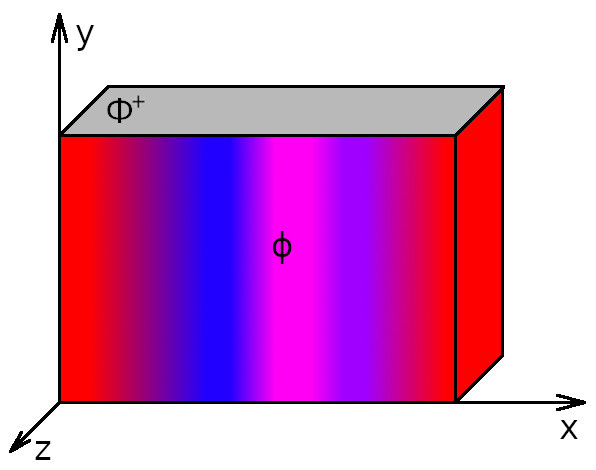
\includegraphics[width=0.85\textwidth]{../figures/one_dim_problem.jpg}
\end{figure}
\end{columns}
\vspace{-0.4cm}
Тогда уравнение на $\phi$ принимает вид
\begin{block}{}
	$$\cfrac{1}{m} \cfrac{\partial \phi}{\partial t} = \cfrac{1}{2} K_\Phi^2 \epsilon'(\phi) +
	\cfrac{\Gamma}{l^2} f'(\phi) + \cfrac{1}{2} \Gamma \cfrac{\partial^2 \phi}{\partial x^2}$$
\end{block}
$K_\Phi = \cfrac{\Phi^+ - \Phi^-}{h}$. Будем считать $\epsilon_0 = \Const$.
\end{frame}


\section{Теоретический анализ}

\begin{frame}{Анализ положений равновесия}
\begin{itemize}
	\item Пробой может развиваться из малых возмущений свойств неповрежденной среды. Выясним
	условия развития.
	\item Рассмотрим положения равновесия вида $\phi(x, t) \equiv C$. Положению равновесия
	соответствует ноль $C$ функции
\end{itemize}
$$\chi(\phi) = \cfrac{1}{2} K_\Phi^2 \epsilon'(\phi) + \cfrac{\Gamma}{l^2} f'(\phi)$$
\vspace{-0.5cm}
\begin{itemize}
	\item Исследуем положения равновесия на устойчивость спектральным методом: к $\phi \equiv C$
	прибавим возмущение $\delta \phi = e^{\alpha t}\cos(\omega x)$, линеаризуем уравнение на
	$\delta \phi$.
	\item $\chi(\phi)$ возрастает в $C \Longrightarrow$ равновесие неустойчиво; $\chi(\phi)$
	убывает в $C \Longrightarrow$ равновесие устойчиво.
\end{itemize}
\end{frame}


\begin{frame}{Анализ положений равновесия}
\vspace{-0.9cm}
\begin{columns}
\column{0.3\textwidth}
\begin{center}
	<<Слабое>> напряжение
\end{center}
\vspace{-0.2cm}
$$0 \leqslant \cfrac{K_\Phi^2 l^2 \epsilon_0}{2 \Gamma} < \delta^2$$
\vspace{-0.7cm}
\begin{figure}
	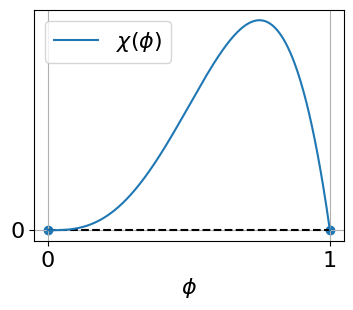
\includegraphics[width=\textwidth]{../figures/equilibriums_case_1.png}
\end{figure}
\column{0.3\textwidth}
\begin{center}
	<<Среднее>> напряжение
\end{center}
\vspace{-0.2cm}
$$\delta^2 < \cfrac{K_\Phi^2 l^2 \epsilon_0}{2 \Gamma} < (1 + \delta)^2$$
\vspace{-0.7cm}
\begin{figure}
	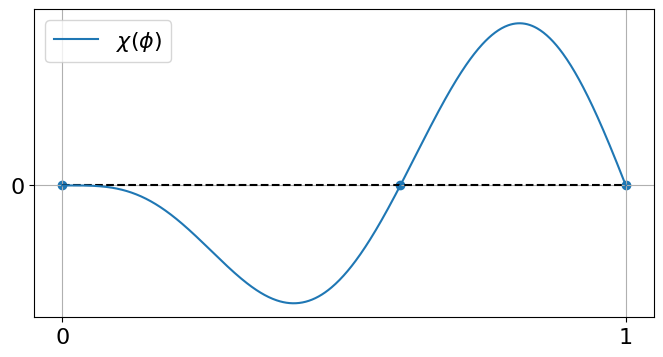
\includegraphics[width=\textwidth]{../figures/equilibriums_case_2.png}
\end{figure}
\column{0.3\textwidth}
\begin{center}
	<<Сильное>> напряжение
\end{center}
\vspace{-0.2cm}
$$(1 + \delta)^2 < \cfrac{K_\Phi^2 l^2 \epsilon_0}{2 \Gamma}$$
\vspace{-0.7cm}
\begin{figure}
	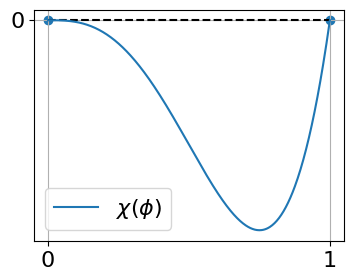
\includegraphics[width=\textwidth]{../figures/equilibriums_case_3.png}
\end{figure}
\end{columns}
\begin{columns}
\column{0.3\textwidth}
\hspace{0.5cm}
$\phi \equiv 0$ неустойчивое \\
\hspace{0.5cm}
$\phi \equiv 1$ устойчивое
\column{0.3\textwidth}
\hspace{0.5cm}
$\phi \equiv 0$ устойчивое \\
\hspace{0.5cm}
$\phi \equiv С_3$ неустойчивое \\
\hspace{0.5cm}
$\phi \equiv 1$ устойчивое
\column{0.3\textwidth}
\hspace{0.5cm}
$\phi \equiv 0$ устойчивое \\
\hspace{0.5cm}
$\phi \equiv 1$ неустойчивое
\end{columns}
\end{frame}


\section{Численный анализ}

\begin{frame}{Разностная схема}
\begin{block}{Разностная задача}
	$$\cfrac{1}{m} \cfrac{\phi_a^{b + 1} - \phi_a^b}{\tau} = \cfrac{1}{2} K_\phi^2
	\epsilon'(\phi_a^b) + \cfrac{\Gamma}{l^2} f'(\phi_a^b) + \cfrac{\Gamma}{2}
	\cfrac{\phi_{a + 1}^b - 2 \phi_a^b + \phi_{a - 1}^b}{h^2}$$
	$$\phi_a^0 = \phi_0(ah); \quad \phi_0^b = \phi_l(b \tau); \quad \phi_{w/h}^b = \phi_r(b \tau)$$
	Сетка регулярная; $\tau$ -- шаг по времени, $h$ -- шаг по пространству.
\end{block}
Явная разностная схема первого порядка по времени, второго -- по пространству.
\end{frame}


\begin{frame}{Оценка устойчивости}
\begin{itemize}
\item Рассмотрим возмущенное решение $\phi_a^b + \delta_a^b$. Линеаризуем уравнение на возмущение
$\delta_a^b$ в точке $\phi_a^b = P$:
\end{itemize}
$$\delta_a^{b + 1} = \delta_a^b + m \tau \left( \cfrac{1}{2} K_\Phi^2 \epsilon''(P) \delta_a^b +
\cfrac{\Gamma}{l^2} f''(P) \delta_a^b + \cfrac{\Gamma}{2} \cfrac{\delta_{a + 1}^b - 2 \delta_a^b +
\delta_{a - 1}^b}{h^2} \right)$$
\begin{itemize}
\item Применим спектральный признак устойчивости:
\end{itemize}
$$1 > \lambda(\theta) = 1 + m \tau \left( \cfrac{1}{2} K_\Phi^2 \epsilon''(P) +
\cfrac{\Gamma}{l^2} f''(P) - \cfrac{2 \Gamma}{h^2} \sin^2 \cfrac{\theta}{2} \right)$$
\begin{itemize}
\item Исследуем вблизи $P = 0$.
\end{itemize}
\end{frame}


\begin{frame}{Оценка устойчивости}
\begin{block}{Условие устойчивости}
	$$\tau \leqslant \cfrac{1}{2m} \left( \cfrac{K_\Phi^2 \epsilon_0}{\delta^{5/3}} +
	\cfrac{\Gamma}{h^2} \right)^{-1}$$
\end{block}
\begin{block}{Упрощенное условие устойчивости}
	$$\tau \leqslant \cfrac{1}{4m} \min \left(\cfrac{\delta^{5/3}}{K_\Phi^2 \epsilon_0}, \;
	\cfrac{h^2}{\Gamma} \right)$$
\end{block}
\end{frame}


\begin{frame}{Вычисления: типичное решение}
\vspace{-0.4cm}
\begin{columns}
\column{0.88\textwidth}
\begin{figure}
	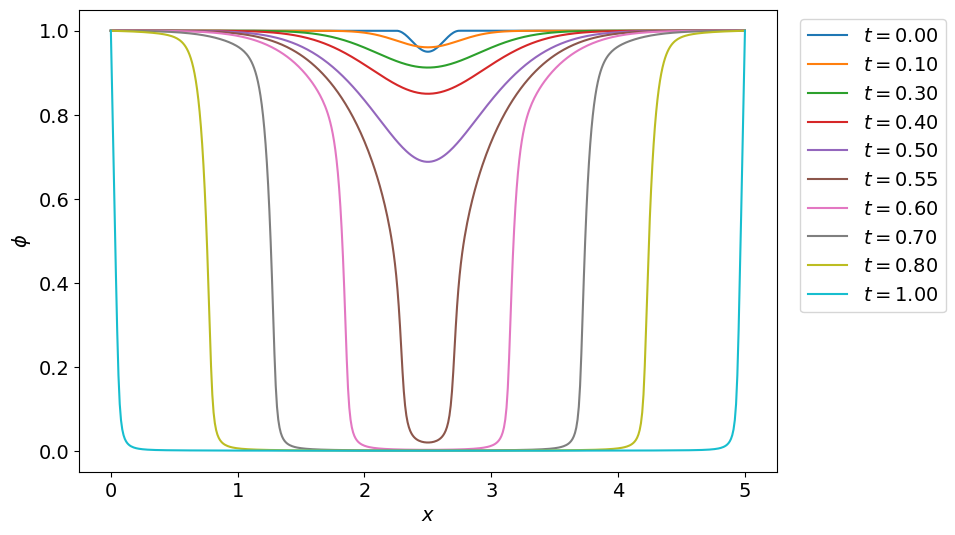
\includegraphics[width=\textwidth]{../figures/typical_solution.png}
\end{figure}
\column{0.12\textwidth}
\hfill \\
\vspace{3.5cm}
\hspace{-2.5cm}
Узлов по измерениям: \\
\hspace{-2.5cm}
$n_x = 10^3, \; n_t = 10^5$
\end{columns}
\end{frame}


\begin{frame}{Вычисления: проверка устойчивости}
\vspace{-0.4cm}
\begin{columns}
\column{0.7\textwidth}
\begin{figure}
	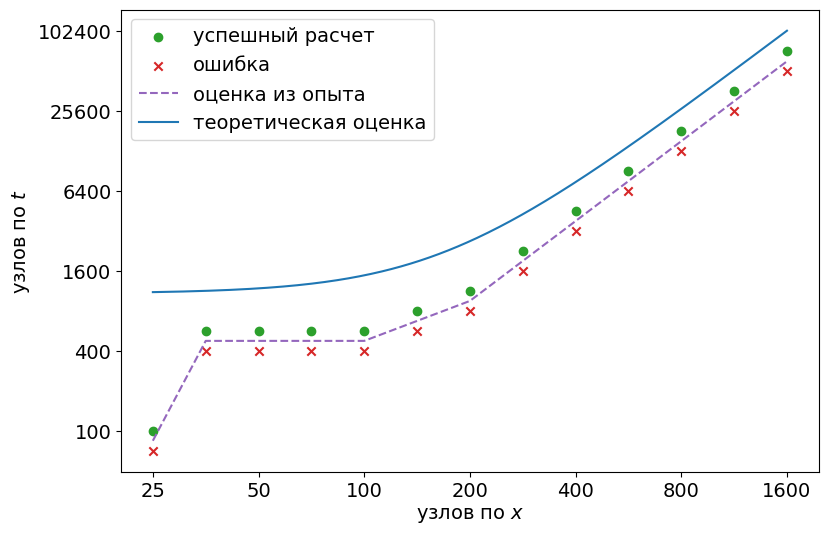
\includegraphics[width=\textwidth]{../figures/stability_bounds.png}
\end{figure}
\column{0.3\textwidth}
$$\tau \leqslant \cfrac{1}{2m} \left( \cfrac{K_\Phi^2 \epsilon_0}{\delta^{5/3}} +
\cfrac{\Gamma}{h^2} \right)^{-1}$$
\end{columns}
\end{frame}


\begin{frame}{Вычисления: проверка сходимости}
\vspace{-0.3cm}
\begin{figure}
	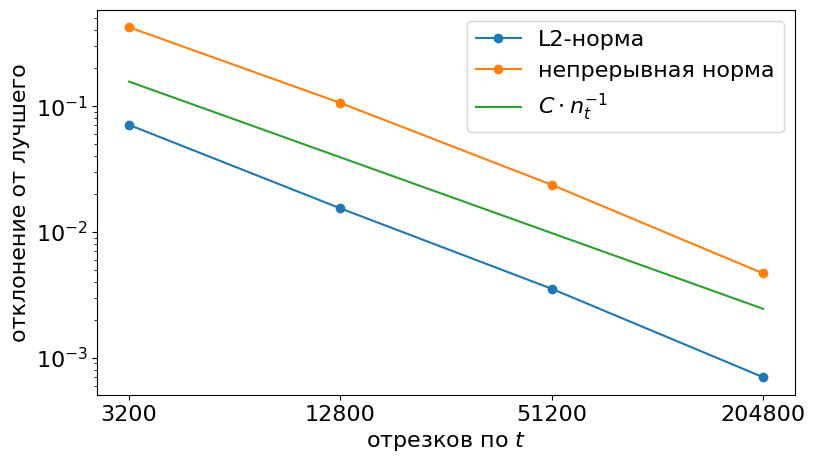
\includegraphics[width=0.58\textwidth]{../figures/convergence_connected.png}
\end{figure}
\vspace{-0.6cm}
\begin{center}
	Здесь, согласно оценке устойчивости, $\tau = \cfrac{h^2}{4m \Gamma}$
\end{center}
\end{frame}


\begin{frame}{Вычисления: положения равновесия}
\vspace{-0.4cm}
\begin{center}
	$(1 + \delta)^2 < \cfrac{K_\Phi^2 l^2 \epsilon_0}{2 \Gamma}$ -- <<сильное>> напряжение
\end{center}
\vspace{-0.4cm}
\begin{columns}
\column{0.5\textwidth}
\begin{figure}
	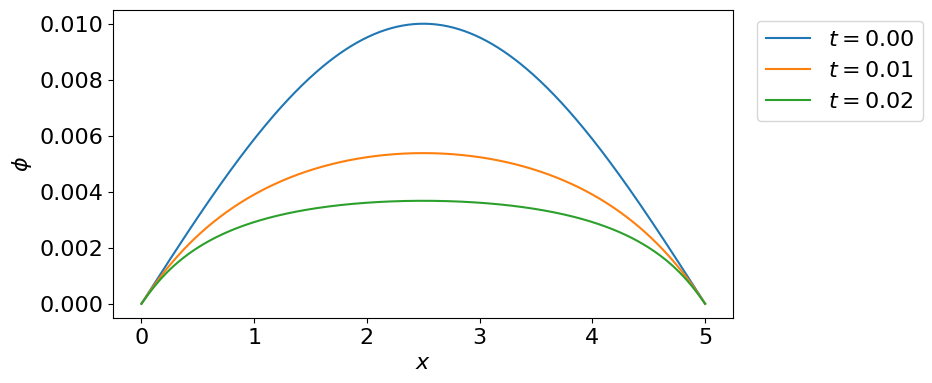
\includegraphics[width=\textwidth]{../figures/equilibrium_3_0.png}
\end{figure}
\vspace{-0.6cm}
\begin{center}
	$\phi \equiv 0$ \\
	устойчивое
\end{center}
\column{0.5\textwidth}
\begin{figure}
	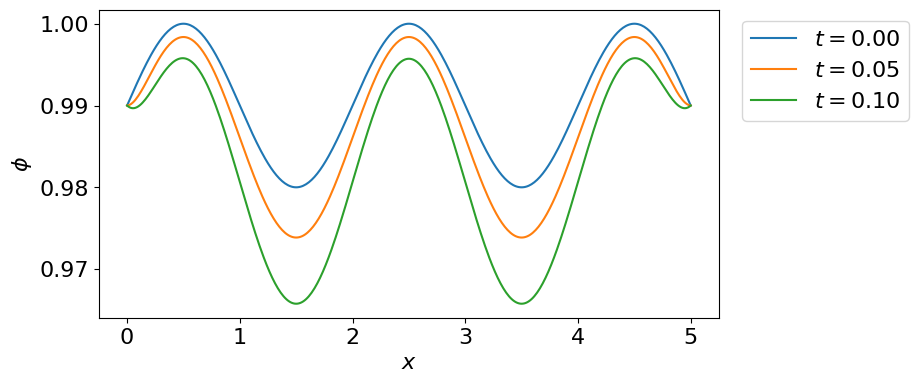
\includegraphics[width=\textwidth]{../figures/equilibrium_3_1.png}
\end{figure}
\vspace{-0.6cm}
\begin{center}
	$\phi \equiv 1$ \\
	неустойчивое
\end{center}
\end{columns}
\end{frame}


\begin{frame}{Свободная энергия}
\vspace{-0.7cm}
$$\Pi(t) = \int\limits_\Omega \pi(x, t) dx$$
$$\pi(x, t) = \pi_1(x, t) + \pi_2(x, t) + \pi_3(x, t)$$
\vspace{-0.3cm}
\begin{itemize}
	\item $\pi_1(x, t) = -\cfrac{K_\Phi^2}{2} \, \epsilon(\phi(x, t))$ -- плотность энергии
	электрического поля;
	\item $\pi_2(x, t) = \Gamma \cfrac{1 - f(\phi(x, t))}{l^2}$ -- плотность энергии, отнесенной
	к веществу внутри канала;
	\item $\pi_3(x, t) = \cfrac{\Gamma}{4} \left( \cfrac{\partial \phi}{\partial x}(x, t)
	\right)^2$ -- плотность энергии, отнесенной к граничной зоне канала
\end{itemize}
\end{frame}


\begin{frame}{Вычисления: свободная энергия}
\vspace{-0.8cm}
\begin{columns}
\column{0.5\textwidth}
\begin{figure}
	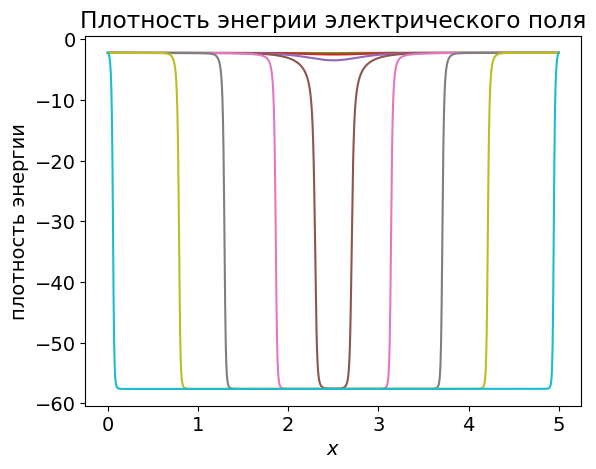
\includegraphics[width=\textwidth]{../figures/density_electrical.png}
\end{figure}
\column{0.5\textwidth}
\begin{figure}
	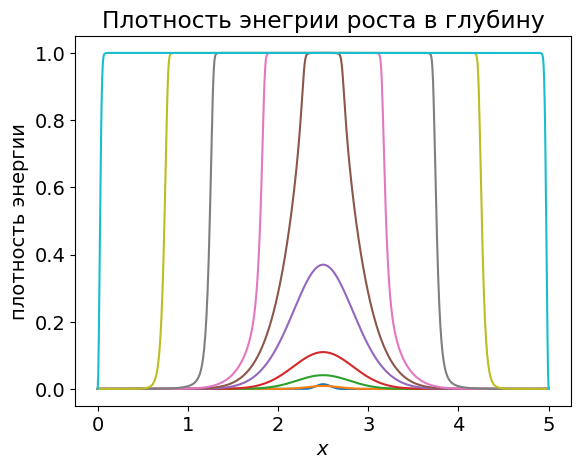
\includegraphics[width=\textwidth]{../figures/density_depth.png}
\end{figure}
\end{columns}
\end{frame}


\begin{frame}{Вычисления: свободная энергия}
\vspace{-0.6cm}
\begin{figure}
	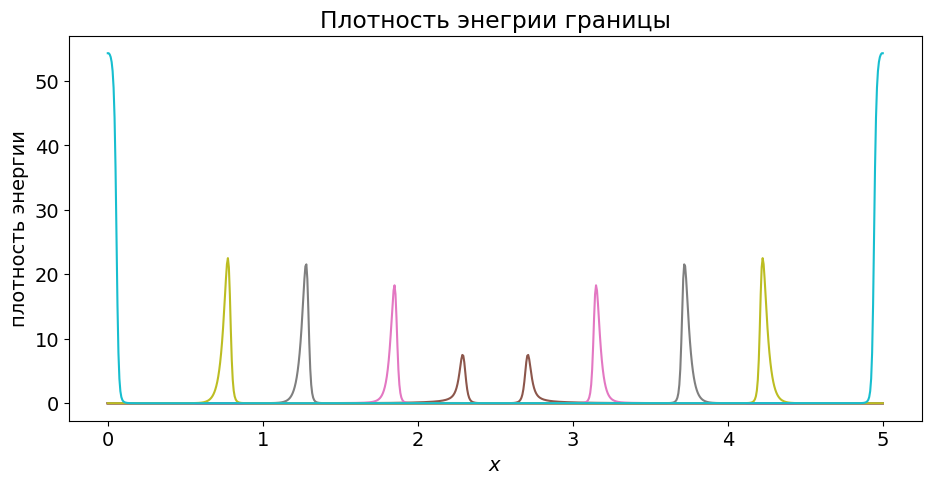
\includegraphics[width=0.86\textwidth]{../figures/density_surface.png}
\end{figure}
\end{frame}


\begin{frame}{Вычисления: свободная энергия}
\vspace{-0.6cm}
\begin{figure}
	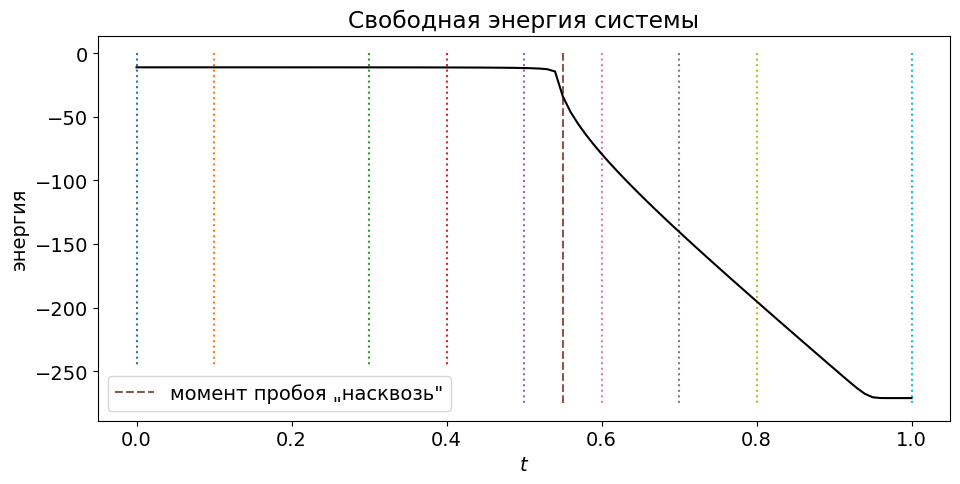
\includegraphics[width=0.88\textwidth]{../figures/energy_total.png}
\end{figure}
\end{frame}


\section{Исследование обобщения модели}

\begin{frame}{Постановка задачи}
Исследуем распределение фазового поля вокруг проводников ($\phi = 0$) различного вида. Рассмотрим
следующие краевые задачи:
\begin{enumerate}
	\item $\Omega = [0, +\infty)_x \times I_y \times I_z, \; \phi|_{x = 0} = 0, \; \phi \to 1$ при
	$r = x \to +\infty$ -- плоский случай;
	\item $\Omega = \mathbb{R}_x \times \mathbb{R}_y \times I_z, \; \phi|_{x, y = 0} = 0, \;
	\phi \to 1$ при $r = \sqrt{x^2 + y^2} \to +\infty$ -- \\ цилиндрический случай;
	\item $\Omega = \mathbb{R}_x \times \mathbb{R}_y \times \mathbb{R}_z, \;
	\phi|_{x, y, z = 0} = 0, \; \phi \to 1$ при $r = \sqrt{x^2 + y^2 + z^2} \to +\infty$ -- \\
	сферический случай.
\end{enumerate}
Ищем стационарное решение $\phi = \phi(r)$.
\end{frame}


\begin{frame}{Суть проблемы}
\begin{columns}
\column{0.5\textwidth}
\centering
Плоский случай
\column{0.5\textwidth}
\centering
Цилиндрический случай
\end{columns}
\vspace{0.5cm}
\begin{columns}
\column{0.49\textwidth}
Задача Коши:
\vspace{-0.3cm}
$$\phi(0) = 0; \qquad \cfrac{\partial \phi}{\partial x} = \cfrac{2}{l} \sqrt{1 - f(\phi)}$$
\begin{figure}
	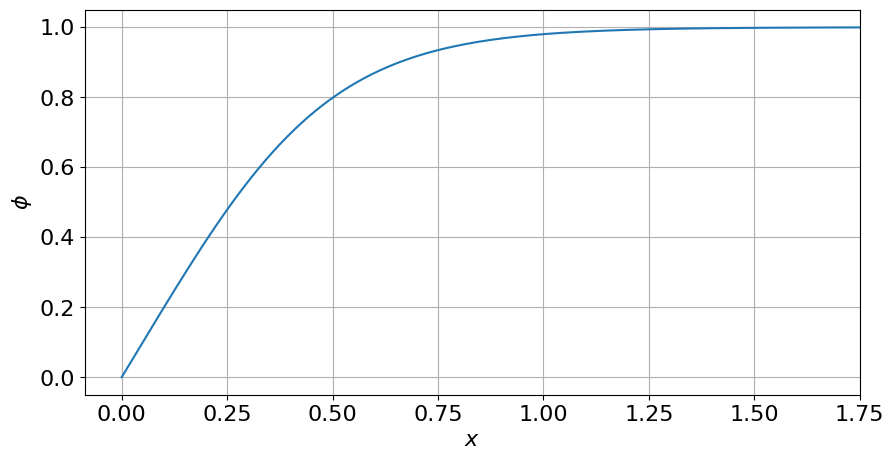
\includegraphics[width=\textwidth]{../figures/result_volumes.png}
\end{figure}
\column{0.01\textwidth}
\rule{0.4pt}{0.7\textheight}
\column{0.49\textwidth}
\centering
Задача поставлена некорректно \\ и решения не имеет \cite{zipunova_higher_codimension}
\end{columns}
\end{frame}


\begin{frame}{Обобщение модели}
\begin{block}{Обобщение модели, предложенное в работе \cite{zipunova_higher_codimension}}
\begin{itemize}
	\item Уравнение электрического потенциала $\Phi$:
	$$\Div(\epsilon[\phi] \nabla \Phi) = 0$$
	\item Уравнение фазового поля $\phi$:
	$$\cfrac{1}{m} \cfrac{\partial \phi}{\partial t} =
    \cfrac{1}{2} \epsilon'(\phi) (\nabla \Phi, \nabla \Phi) +
    \cfrac{\Gamma}{l^2} f'(\phi) +
    \cfrac{1}{2} \Gamma \triangle \phi -
    \alpha \cfrac{\Gamma l^2}{4} \triangle^2 \phi +
    \beta \Gamma l^{p - 2} \Div (\| \, \nabla \phi \, \|_2^{p - 2} \nabla \phi)$$
\end{itemize}
\end{block}
\begin{itemize}
	\item $\triangle^2 \phi = \triangle(\triangle \phi)$ -- билапласиан;
	\item $\Div (\| \, \nabla \phi \, \|_2^{p - 2} \nabla \phi)$ -- $p$-лапласиан
\end{itemize}
\end{frame}


\begin{frame}{Разностная схема}
На границе $r = 0$ области моделирования у решения $\phi$ ожидается особенность. \\
Основная идея: пусть одна из базисных функций, используемых для приближения $\phi$ вблизи $0$,
имеет тот же вид особенности.
$$\cfrac{1}{m} (\widetilde{\phi}_i^{j + 1} - \widetilde{\phi}_i^j) = \tau \cfrac{\Gamma}{l^2}
f'(\widetilde{\phi}_i^j) + \cfrac{\tau}{dV_i} \Gamma (\rho_{i + 1/2}^j S_{i + 1/2} -
\rho_{i - 1/2}^j S_{i - 1/2}) \text{;}$$
$$dV_i = r_{i + 1/2}^{k + 1} - r_{i - 1/2}^{k + 1}; \qquad
S_{i \pm 1/2} = (k + 1) r_{i \pm 1/2}^k \text{;}$$
$$\rho_{i \pm 1/2}^j = \cfrac{1}{2}
\left[ \cfrac{\partial \phi}{\partial r} \right]_{i \pm 1/2}^j -
\alpha \cfrac{l^2}{4} \left[ \cfrac{\partial (\triangle \phi)}{\partial r} \right]_{i \pm 1/2}^j +
\beta l^2 \left( \left[ \cfrac{\partial \phi}{\partial r} \right]_{i \pm 1/2}^j \right)^3
\text{;}$$
$$\widetilde{\triangle \phi}_i^j = \cfrac{1}{dV_i}
\left( \left[ \cfrac{\partial \phi}{\partial r} \right]_{i + 1/2}^j S_{i + 1/2} -
\left[ \cfrac{\partial \phi}{\partial r} \right]_{i - 1/2}^j S_{i - 1/2} \right)$$
\end{frame}


\begin{frame}{Полученные результаты}
\vspace{-1cm}
\begin{center}
	Предполагаемые виды особенности решения $\phi$ в точке $r = 0$
\end{center}
\begin{tabular}{|m{3cm}||m{3.5cm}|m{3.5cm}|m{3.5cm}|}
	\hline
	\vspace*{2mm} \hfill \vspace*{2mm} &\centering $\alpha = 0, \; \beta = 0$ &
	\centering $\alpha = 0, \; \beta \neq 0$ & \centering \arraybackslash $\alpha \neq 0$ \\
	\hline
	\hline
	\vspace{2mm} Плоский \linebreak случай \vspace{2mm} &
	Без особенности & Без особенности & Без особенности \\
	\hline
	\vspace{2mm} Цилиндрический \linebreak случай \vspace{2mm} &
	Не имеет решения & $r^{2/3}$ & $r^2 (\ln r - 1)$ \\
	\hline
	\vspace{2mm} Сферический \linebreak случай \vspace{2mm} &
	Предположительно не имеет решения & $r^{1/3}$ & Предположительно
	не имеет решения \\
	\hline
\end{tabular}
\end{frame}


\begin{frame}{Полученные результаты}
\vspace{-0.6cm}
\begin{figure}
	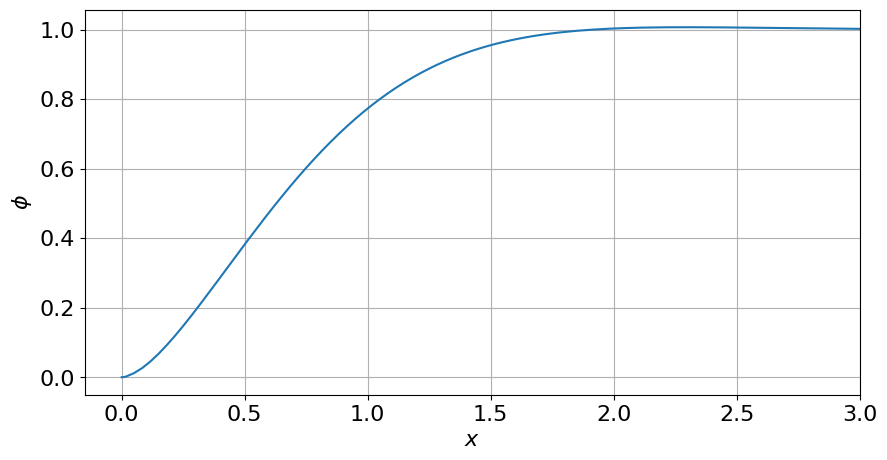
\includegraphics[width=0.81\textwidth]{../figures/result_volumes_cyl_bi.png}
\end{figure}
\vspace{-0.7cm}
\begin{center}
	Цилиндрический случай, $\alpha = 1$: особенность вида $r^2 (\ln r - 1)$
\end{center}
\end{frame}


\begin{frame}{Полученные результаты}
\vspace{-0.6cm}
\begin{figure}
	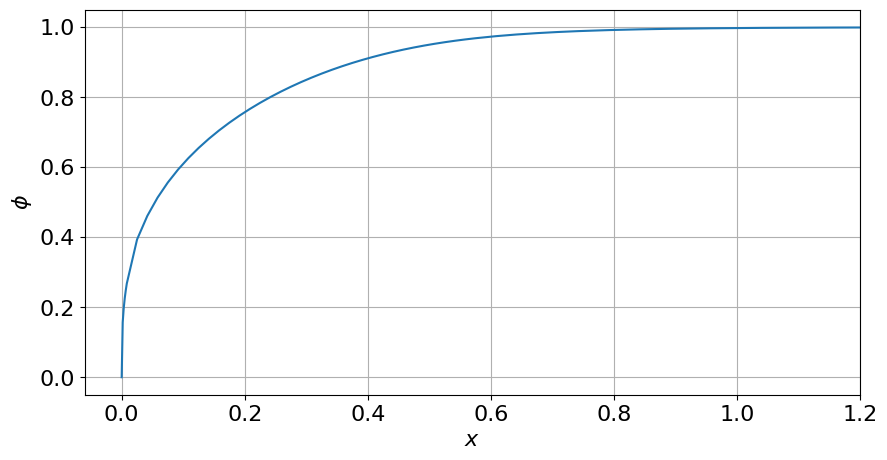
\includegraphics[width=0.81\textwidth]{../figures/result_volumes_sph_p.png}
\end{figure}
\vspace{-0.7cm}
\begin{center}
	Сферический случай, $\alpha = 0, \; \beta = 1$: особенность вида $r^{1/3}$
\end{center}
\end{frame}


\begin{frame}{Заключение}
Основные результаты работы.
\begin{itemize}
    \item Проведен теоретический анализ модели.
    \item Построена разностная схема, дана содержательная оценка ее устойчивости.
    \item Исследовано обобщение исходной модели; на основе метода конечных объемов построена
    специальная разностная схема, учитывающая особенности решений на границе области моделирования.
\end{itemize}
\end{frame}


\begin{frame}{Литература}
\printbibliography
\end{frame}


\begin{frame}{}
\begin{center}
	\Large
	Спасибо за внимание
\end{center}
\end{frame}


\end{document}